%% Manuscript for the IEEE Internet of Things Journal, IEEEtran class (two columns).
%% Build: latexmk -pdf ieee_main.tex   (from the paper/ directory)
\documentclass[journal]{IEEEtran}
% Packages and macros shared by the JNCA (elsarticle) and IEEE IoT-J (IEEEtran) versions.
\usepackage{amsmath,amssymb}
\usepackage{graphicx}
\usepackage{booktabs}
\usepackage{array}
\usepackage{tabularx}
\usepackage{enumitem}
\usepackage{xcolor}
\usepackage{pifont}
\usepackage{tikz}
\usetikzlibrary{arrows.meta,positioning}
\usepackage{algorithm}
\usepackage{algpseudocode}
\usepackage{url}
\usepackage[hidelinks]{hyperref}

\newcommand{\cmark}{\ding{51}}            % provided
\newcommand{\xmark}{\ding{55}}            % not provided / not reported
\newcommand{\pmark}{$\sim$}              % partly
\renewcommand{\tabularxcolumn}[1]{p{#1}}
\makeatletter
\newcommand{\inputtab}[1]{\@@input #1 }   % \input that works inside a tabular (generated table rows)
\makeatother
\newcolumntype{L}[1]{>{\raggedright\arraybackslash}p{#1}}

\newenvironment{widetab}{\begin{table*}[tp]}{\end{table*}}   % two columns: wide tables span both
\begin{document}

\title{Does Energy-Efficient WSN Routing Need Learning? A Benchmark Against the Provable Optimum and a Coordinated Dijkstra Over a Shared Load Table}

%% AUTHORS: replace the placeholders.
\author{[Author 1], [Author 2], and [Supervisor]%
\thanks{The authors are with the [Department], Netaji Subhas University of Technology, New Delhi 110078, India (e-mail: [email]).}}

\maketitle

\begin{abstract}
Deep reinforcement learning is increasingly proposed for energy-efficient routing in wireless sensor networks (WSNs), but learned routers are rarely compared with strong classical baselines or with the achievable optimum. We score every method against a provable lifetime ceiling, the Chang--Tassiulas maximum-lifetime linear program, and an oracle version for time-varying traffic. On held-out deployments in the setting of a recent multi-agent deep reinforcement learning router (MADII, IEEE Internet of Things Journal, 2025), MADII reaches 11\% of the ceiling. Battery-weighted Dijkstra reaches 88\% with no training, and reinforcement learning warm-started from it adds nothing significant. We then propose LEST load-table Dijkstra, a solver-free coordinated router. Each round the sink builds the routing tree node by node, nearest the sink first, and charges every relay for the traffic already booked through it in that round. Exact batteries are combined with node loads shared as 4-tier entries piggybacked on existing packets, and this overhead is charged in the energy model. Under four time-varying traffic scenarios it reaches 90.5\% of the oracle, against 85.0\% for battery-weighted Dijkstra (118 of 120 deployments won; Wilcoxon $p<10^{-20}$). A published energy-and-load router (EBR-DA) reaches 15\%. An LP planner re-solved every round reaches 97.0\% and serves as an upper reference; a traffic forecast adds only 0.5 points to it. The ranking holds on event-driven traffic derived from the Intel Berkeley Lab dataset (MADII 11.8\%, battery Dijkstra 86.0\%, LEST Dijkstra 90.8\%, LP planner 96.9\%).

\end{abstract}

\begin{IEEEkeywords}
Wireless sensor networks, network lifetime, energy-efficient routing, load balancing, maximum-lifetime linear program, deep reinforcement learning, Internet of Things.
\end{IEEEkeywords}

\section{Introduction}\label{sec:intro}

A wireless sensor network (WSN) consists of battery-powered nodes that sense their surroundings and forward readings to a sink, usually over several hops. Every packet a node sends or relays costs energy, and once the first node is exhausted part of the network can be cut off. The number of rounds until the first node dies (FND) is therefore a standard measure of network lifetime~\cite{chang2004maximum}, and lifetime-aware routing is a central design problem in WSNs and in the low-power Internet of Things (IoT).

A growing line of work applies deep reinforcement learning (DRL) to this problem: neural networks learn to choose next hops, cluster heads or transmit powers~\cite{yang2025madii,younus2021sdwsn,tang2025twotier}. These methods need long training and often a GPU. They are usually evaluated against clustering heuristics, metaheuristics or other learned methods. We found no recent learned WSN router that was compared with a battery-weighted shortest-path router, and none that reported its lifetime as a fraction of a provable optimum. Recent comparison studies even tabulate published results obtained on different datasets and in different units~\cite{icmcsi2026}. As a result, it is hard to tell how much the learning contributes. Neighbouring areas of networking show the same pattern: simple, well-tuned baselines match deep models once they are evaluated carefully~\cite{simplemodel2025}.

This paper answers the question by measurement. The maximum-lifetime linear program (LP) of Chang and Tassiulas~\cite{chang2004maximum} gives a ceiling that no routing scheme can exceed. For traffic that varies over time we use an oracle version that knows all future traffic. Every method is scored as the percentage of that ceiling it reaches, on held-out deployments and on real traffic. Against this yardstick the methods separate into clear levels. A recent multi-agent DRL router, MADII~\cite{yang2025madii}, rebuilt in its own published setting, reaches about 11--15\% of the ceiling. A published energy-and-load router, EBR-DA~\cite{mahdi2018ebrda}, reaches about 15\%. Battery-weighted Dijkstra reaches 85--88\% with no training.

The remaining gap comes from coordination: in battery-weighted Dijkstra every node picks its path independently, so in the same round many nodes can pick the same relay. We propose \emph{LEST load-table Dijkstra}, a solver-free router that closes about half of the gap. Each round the sink builds the routing tree one node at a time, nearest the sink first. Each node's path is found by Dijkstra over a link cost that combines radio energy, the exact residual battery and the load already booked on each relay in that round. Each source's traffic rate reaches the sink through a Lightweight State Table (LEST): every node reports its load as one of four tiers, piggybacked on packets it already sends. Finally, an LP planner re-solved every round from live batteries serves as an upper reference for what full flow optimisation adds.

\paragraph{Contributions} The contributions of this paper are:
\begin{enumerate}[label=(C\arabic*), leftmargin=*]
  \item \textbf{An oracle-normalised benchmark for lifetime routing.} Every method is reported as a percentage of a provable ceiling: the maximum-lifetime LP for static traffic, and an oracle LP, solved by bisection, for time-varying traffic. The benchmark covers 30 held-out deployments per scenario, four traffic scenarios, real event-driven traffic from the Intel Berkeley Lab dataset~\cite{intellab2004} and paired Wilcoxon tests with Holm correction.
  \item \textbf{A measured ranking of learned, published and classical routers.} MADII, rebuilt in its own setting and checked against its published figures, reaches 11.1\% of the ceiling (19.5 rounds against the paper's 19). Battery-weighted Dijkstra reaches 88.4\%, and DRL warm-started from Dijkstra adds no significant gain ($p=0.24$).
  \item \textbf{LEST load-table Dijkstra.} A per-round, solver-free and training-free router that builds the tree sequentially with within-round load booking, using exact energy and a 4-tier shared load table whose overhead is charged in the energy model. It reaches 90.5\% of the oracle against 85.0\% for battery-weighted Dijkstra (118/1/1 wins, ties and losses over 120 deployments) and 90.8\% against 86.0\% on Intel Lab traffic.
  \item \textbf{Ablations and negative results.} Both the energy term and the load term are needed (load only 45.1\%, energy only 85.0\%, both 90.5\%), and energy must stay exact rather than tiered. Five ways of adding prediction, lifetime weighting or LP prices to Dijkstra stay within about $\pm1$ point of it. A Holt-Winters forecast adds only 0.5 points to an LP planner that is re-solved every round.
\end{enumerate}
All code, the result files and the scripts that generate every table and figure are released (see the data availability statement).

Section~\ref{sec:related} reviews related work and positions this paper. Section~\ref{sec:model} states the system model, the packet-layer model and every assumption. Section~\ref{sec:methods} describes the proposed router and the reference methods, and Section~\ref{sec:setup} the evaluation protocol. Section~\ref{sec:results} reports the results and the statistical tests, Section~\ref{sec:discussion} discusses them together with the threats to validity, and Section~\ref{sec:conclusion} concludes.

\section{Related work and literature survey}\label{sec:related}

\subsection{Energy models and clustering}
Heinzelman et al.~\cite{heinzelman2000leach} introduced the first-order radio model that most WSN routing studies use, including ours (Section~\ref{sec:radio}). In it, transmitting costs electronics energy plus an amplifier term that grows with the square or the fourth power of distance, and receiving costs electronics energy only. Their LEACH protocol popularised clustering with rotating cluster heads. Later schemes select cluster heads with fuzzy c-means (FCM) or with population metaheuristics such as grey-wolf/whale hybrids, the honey badger algorithm (HBA) and the pelican optimisation algorithm (POA). These are the baselines against which MADII is evaluated~\cite{yang2025madii}.

\subsection{Lifetime-optimal and energy-aware shortest-path routing}
Dijkstra's algorithm~\cite{dijkstra1959note} finds least-cost paths for given link costs. With radio energy as the cost it gives minimum-total-energy (MTE) routing, which is optimal for one round but exhausts the same relays first. Chang and Tassiulas~\cite{chang2004maximum} formulated maximum-lifetime routing as an LP over link flows. Because the LP allows fractional, time-shared routing, its optimum is an upper bound on the lifetime of any routing scheme, and we use it as the ceiling. They also proposed flow augmentation: shortest paths over link costs that combine energy per bit with the residual energy at both ends, recomputed as flow is added. They reported lifetimes close to the LP optimum and compared against MTE routing. The battery-weighted Dijkstra baseline in this paper is the single-tree, per-round member of that family. Recent theoretical progress on single-source shortest paths~\cite{duan2025sorting} computes the same paths asymptotically faster. It cannot change routing quality, and at WSN sizes the cost of Dijkstra itself is negligible (Section~\ref{sec:computation}).

\subsection{Load-balanced routing trees}
Traffic funnels towards the sink, so the nodes next to it relay the most and die first. Dai and Han~\cite{dai2003nodecentric} proposed a node-centric algorithm that grows a tree from the sink, repeatedly grafting the heaviest unassigned border node onto the lightest branch. As described in~\cite{shan2013lifetime}, it balances load but ignores distance and energy. Shan et al.~\cite{shan2013lifetime} construct a load-balanced \emph{shortest-path} spanning tree, in which every sensor reaches the sink in its minimum hop count. Their top-down network-flow construction is followed by distributed balance refinement, and they report lifetimes of about 85\% of an upper bound. Both build one tree under uniform initial energy; neither rebuilds it from residual batteries. EBR-DA~\cite{mahdi2018ebrda} combines residual energy and buffer occupancy in a node weight over a hop tree, and each node forwards to its lightest neighbour one hop nearer the sink. It is evaluated in MATLAB against DRINA and InFRA, two aggregation-oriented protocols, with no optimum bound. Combining energy and load in a routing cost, and building load-balanced trees, are therefore not new. What we add is the per-round rebuild with exact battery weighting, the within-round booking order, the LEST sharing with charged overhead, and the measurement against the optimum. Our ablations (Section~\ref{sec:ablation}) show that the load term alone, close in spirit to load-only trees, reaches only 45\% of the oracle.

\subsection{Learning-based routing and energy control}
Tang et al.~\cite{tang2025twotier} propose a two-tier system for low-power mesh networks: a central reinforcement-learning coordinator plus small neural networks on each node that adjust transmit power. MADII~\cite{yang2025madii} is a multi-agent deep Q-network~\cite{mnih2015dqn} with an Informer encoder~\cite{zhou2021informer}, which picks the next hop of every sensor under centralised training and centralised execution. It is trained first from clustering algorithms through imitation and then by exploration, and reports gains over FCM, GWO-WOA, HBA, POA and learned ablations. The full text contains no shortest-path baseline and no optimum bound. Younus et al.~\cite{younus2021sdwsn} train an RL agent inside a software-defined WSN controller that has the global network view. Their testbed evaluation compares the agent with an RL-based WSN routing scheme and reports a 23--30\% longer lifetime. A recent review of learning for routing~\cite{learning4routing2025} surveys the broader trend. In each case the learned method is compared with heuristics or other learners, not with battery-weighted shortest paths or the optimum.

\subsection{Forecasting and algorithms with predictions}
Holt-Winters exponential smoothing~\cite{holt2004forecasting,winters1960forecasting} forecasts series with level, trend and seasonal components, and it remains a strong baseline for periodic data such as daily sensor traffic. Work on algorithms with predictions~\cite{lykouris2018caching} studies classical algorithms that take a forecast as advice. It asks how much they gain when the forecast is right and how much they lose when it is wrong. We follow this framing when we test forecasts inside Dijkstra and inside an LP planner (Section~\ref{sec:prediction}).

\subsection{Literature survey and research gap}
Table~\ref{tab:survey} summarises the closest studies. Table~\ref{tab:ticks} compares their characteristics with this work: what each router uses to decide, and how each study is evaluated. A recent comparison paper~\cite{icmcsi2026} illustrates the evaluation gap. It tabulates the published results of about ten methods on two different datasets, in units ranging from joules to percentages, with no common simulator, no shortest-path baseline and no optimum. The gap that this paper fills is first one of measurement: learned and heuristic WSN routers are published without reference to the simplest strong classical router or to the achievable lifetime. It is second one of method: no solver-free router that we know of combines exact battery weighting with load booked within the round and a shared tiered load table, re-plans every round, and charges its own overhead.

\begin{widetab}
\centering
\caption{Literature survey of the closest work.}\label{tab:survey}
\scriptsize\renewcommand{\arraystretch}{1.25}
\begin{tabularx}{\textwidth}{@{}>{\raggedright\arraybackslash}p{2.3cm}>{\raggedright\arraybackslash}p{1.7cm}>{\raggedright\arraybackslash}X>{\raggedright\arraybackslash}p{2.1cm}>{\raggedright\arraybackslash}X@{}}
\toprule
Work (year) & Category & Approach & Compared with & Gap relative to this work\\
\midrule
Heinzelman et al.~\cite{heinzelman2000leach} (2000) & Clustering & LEACH; first-order radio model & Direct, MTE & No optimum; clustering rather than multi-hop routing to a sink\\
Dai and Han~\cite{dai2003nodecentric} (2003) & Load-balanced tree & Node-centric grafting of heavy nodes onto light branches & -- (as described in~\cite{shan2013lifetime}) & Load only; no energy or distance; one tree\\
Chang and Tassiulas~\cite{chang2004maximum} (2004) & Lifetime-optimal routing & Max-lifetime LP; flow augmentation over energy-and-residual link costs & LP optimum, MTE & No real data, overhead or statistical tests; table-driven\\
Shan et al.~\cite{shan2013lifetime} (2013) & Load-balanced tree & Load-balanced shortest-path tree by network flow plus refinement & Node-centric~\cite{dai2003nodecentric}, upper bound & One static tree; uniform energy; min-hop constraint\\
Mahdi et al., EBR-DA~\cite{mahdi2018ebrda} (2018) & Energy + load routing & Hop tree; node weight $0.6(1-E/E_0)^2+0.4\,\mathrm{buffer}^2$ & DRINA, InFRA & No optimum or shortest-path baseline; designed for aggregation\\
Younus et al.~\cite{younus2021sdwsn} (2021) & Learned (SDWSN) & RL in a controller with a global view; four rewards & RL-based WSN routing & No classical baseline or optimum; testbed only\\
Tang et al.~\cite{tang2025twotier} (2025) & Learned power control & Central RL coordinator plus per-node networks & -- & Power control rather than routing; no optimum\\
Yang et al., MADII~\cite{yang2025madii} (2025) & Learned routing & Multi-agent DQN with Informer; imitation then exploration & FCM, GWO-WOA, HBA, POA, ablations & No shortest-path baseline or optimum; constant traffic\\
ICMCSI study~\cite{icmcsi2026} (2026) & Comparison & Tabulates ten published methods on two datasets & Published numbers & Mixed units; no common simulator or bound\\
Duan et al.~\cite{duan2025sorting} (2025) & Shortest-path theory & SSSP faster than sorting-bound Dijkstra & Theory & Same paths, so no change to lifetime\\
\midrule
This work & Benchmark + coordinated routing & Oracle-normalised bench; LEST load-table Dijkstra; LP planner & Optimum, battery Dijkstra, MADII, EBR-DA & --\\
\bottomrule
\end{tabularx}
\end{widetab}

\begin{widetab}
\centering
\caption{Characteristics of the closest work and of this work. \cmark: provided; \pmark: partly; \xmark: not provided or not reported. Method columns describe what the router uses to decide; evaluation columns describe the study.}\label{tab:ticks}
\footnotesize
\setlength{\tabcolsep}{3pt}
\begin{tabularx}{\textwidth}{@{}X cccccc cccccc@{}}
\toprule
& \multicolumn{6}{c}{Method} & \multicolumn{6}{c}{Evaluation}\\
\cmidrule(lr){2-7}\cmidrule(l){8-13}
Work & M1 & M2 & M3 & M4 & M5 & M6 & E1 & E2 & E3 & E4 & E5 & E6\\
\midrule
Chang and Tassiulas~\cite{chang2004maximum} & \cmark & \pmark & \pmark & \cmark & \cmark & \cmark & \cmark & \xmark & \cmark & \cmark & \xmark & \xmark\\
Shan et al.~\cite{shan2013lifetime} & \xmark & \cmark & \cmark & \xmark & \cmark & \pmark & \xmark & \pmark & \pmark & \cmark & \xmark & \xmark\\
EBR-DA~\cite{mahdi2018ebrda} & \cmark & \cmark & \xmark & \cmark & \cmark & \cmark & \pmark & \xmark & \xmark & \xmark & \xmark & \xmark\\
Younus et al.~\cite{younus2021sdwsn} & \cmark & \cmark & \pmark & \cmark & \xmark & \cmark & \xmark & \pmark & \xmark & \xmark & \cmark & \xmark\\
MADII~\cite{yang2025madii} & \cmark & \cmark & \pmark & \cmark & \xmark & \cmark & \xmark & \pmark & \xmark & \xmark & \xmark & \xmark\\
\midrule
Battery-weighted Dijkstra (baseline, this work) & \cmark & \xmark & \xmark & \cmark & \cmark & \cmark & \cmark & \cmark & \cmark & \cmark & \cmark & \cmark\\
LP planner (upper reference, this work) & \cmark & \cmark & \cmark & \cmark & \cmark & \xmark & \cmark & \cmark & \cmark & \cmark & \cmark & \cmark\\
\textbf{LEST load-table Dijkstra (proposed)} & \cmark & \cmark & \cmark & \cmark & \cmark & \cmark & \cmark & \cmark & \cmark & \cmark & \cmark & \cmark\\
\bottomrule
\end{tabularx}

\smallskip
\raggedright\footnotesize
M1 residual energy in the route decision; M2 relay load in the route decision; M3 within-round coordination (a node's choice accounts for the choices of others in the same round); M4 re-planned from the current state every round; M5 no offline training; M6 no optimisation solver at run time.\\
E1 time-varying traffic evaluated; E2 control overhead charged in the energy model; E3 compared with a shortest-path baseline; E4 compared with a provable optimum; E5 real data or testbed (for this work, real Intel Lab traffic traces); E6 statistical significance tests.
\end{widetab}

\section{System model and assumptions}\label{sec:model}

\subsection{Network model}
The network has $n$ static sensor nodes $V=\{1,\dots,n\}$ and one sink $s$. In the main setting, which is MADII's published setting~\cite{yang2025madii}, $n=100$ nodes are placed uniformly at random in a $500\times500$~m field with the sink at the centre. Every node starts with energy $E_0$. Time is divided into rounds. In round $t$ node $i$ generates $k_i(t)$ packets of $L$ bits, and every packet is forwarded to the sink along the round's routing tree, described by a parent function $p_t:V\to V\cup\{s\}$. Relays forward everything they receive, with no aggregation. The network lifetime $T$ is the number of rounds until the first node exhausts its battery (FND). We also report the rounds until 10\%, 25\% and 50\% of the nodes are dead, the data delivered, energy efficiency (kbit delivered per joule) and hops per packet.

\subsection{Radio energy model}\label{sec:radio}
Transmitting $k$ bits over distance $d$ and receiving $k$ bits cost
\begin{align}
E_{\mathrm{TX}}(k,d) &= \begin{cases} k E_{\mathrm{elec}} + k\,\varepsilon_{\mathrm{fs}} d^2, & d<d_0,\\ k E_{\mathrm{elec}} + k\,\varepsilon_{\mathrm{amp}} d^4, & d\ge d_0,\end{cases}\label{eq:tx}\\
E_{\mathrm{RX}}(k) &= k E_{\mathrm{elec}}, \qquad d_0=\sqrt{\varepsilon_{\mathrm{fs}}/\varepsilon_{\mathrm{amp}}}\approx 87.7~\mathrm{m}.\label{eq:rx}
\end{align}
We write $e_{\mathrm{tx}}(i,j)=E_{\mathrm{TX}}(1,d_{ij})$ and $e_{\mathrm{rx}}=E_{\mathrm{elec}}$ for the per-bit costs. Table~\ref{tab:params} lists the parameters.

\begin{table}[t]
\centering
\caption{Network, radio and packet parameters (MADII's Table~I~\cite{yang2025madii}).}\label{tab:params}
\footnotesize
\begin{tabularx}{\linewidth}{@{}L{0.4\linewidth}X@{}}
\toprule
Parameter & Value\\
\midrule
Sensors, field, sink & 100, uniform in $500\times500$~m, centre\\
Initial energy $E_0$ & 0.5~J (Intel Lab bench: 1.0 and 1.5~J)\\
Data packet $L$ & 4{,}000 bits\\
Route advertisement $L_c$ & 100 bits per round, to every node\\
$E_{\mathrm{elec}}$ & 50~nJ/bit\\
$\varepsilon_{\mathrm{fs}}$ / $\varepsilon_{\mathrm{amp}}$ & 10~pJ/bit/m$^2$ / 0.0013~pJ/bit/m$^4$\\
Crossover distance $d_0$ & 87.7~m\\
Aggregation at relays & None (full forwarding)\\
LEST load report & +8 bits on each data packet\\
LEST snapshot & +2 bits per node in the advertisement\\
\bottomrule
\end{tabularx}
\end{table}

\subsection{Packet-layer model}\label{sec:packet}
The study is round-based rather than slot-based, but every bit a router adds is charged at the packet layer, so the routers pay for their own coordination. Three packet types exist:
\begin{enumerate}[label=(\roman*), leftmargin=*]
  \item \textbf{Data packets} of $L=4{,}000$ bits. Each packet is sent hop by hop to the sink. At every hop the sender pays $E_{\mathrm{TX}}(L,d)$ and the receiver $E_{\mathrm{RX}}(L)$.
  \item \textbf{The route advertisement}, a broadcast of $L_c=100$ bits that the sink sends once per round. Every alive node pays $E_{\mathrm{RX}}(L_c)$ to receive its next hop. This is the control cost MADII's setting already charges, and it is identical for every method.
  \item \textbf{LEST traffic}, charged only to the LEST router. Each data packet carries an extra byte holding the sender's load report, so $L$ becomes $4{,}008$ bits for every hop of every packet. The advertisement carries the snapshot of all load tiers, 2 bits per node, so $L_c$ becomes $100+2n=300$ bits at $n=100$.
\end{enumerate}
A relay that cannot afford a transmission dies within the round, and the packets routed through it in that round are lost. A source whose path fails retries directly to the sink if its battery allows. The delivery ratio is reported with the results (Table~\ref{tab:traffic}). No acknowledgements, retransmissions or MAC frames are modelled, and the MAC is assumed to schedule transmissions without collisions; see assumption A5 below. This is MADII's idealisation, and we keep it so that the comparison is made on MADII's own terms.

\subsection{Traffic models}\label{sec:traffic}
\paragraph{Static traffic} Every node sends one packet per round, $k_i(t)=1$, as in MADII.
\paragraph{Time-varying traffic} One day is 24 rounds, and every method gets 3 days of pre-deployment history. There are four scenarios:
\begin{itemize}[leftmargin=*]
  \item \textbf{Daily surge (R).} The 20\% of nodes nearest a random point form a hotspot. They send Poisson traffic with mean 4 packets per round during a 6-round evening and 0.5 otherwise; all other nodes have mean 1.
  \item \textbf{Constant (N).} $k_i(t)=1$ for every node and round.
  \item \textbf{Bursts (B).} R plus random bursts: each round, with probability 0.05, a random node sends five times its rate for 4 rounds.
  \item \textbf{Pattern shift (D).} R with the hotspot moved to 20 different nodes after two days. D is reported as a robustness test, and nothing is tuned on it.
\end{itemize}
\paragraph{Real traffic (Intel Berkeley Lab)} The Intel Lab dataset~\cite{intellab2004} holds about 2.3 million readings from 54 motes. Traffic is derived by send-on-delta reporting with one-hour rounds. Each mote sends one heartbeat per hour, plus one packet whenever its temperature or light has moved by more than 0.5~$^\circ$C or 100~lux since its last report. This gives about 3.4 packets per mote-hour, and the busiest hour carries 6.6 times the traffic of the quietest. Readings from motes below 2.4~V or with temperatures outside 0--50~$^\circ$C are dropped. The 31 days before most motes died are used. The real mote layout ($40\times31$~m) is scaled by 12 to MADII's field, because at lab scale the direct link to the sink is almost always cheapest.

\subsection{Assumptions}\label{sec:assumptions}
All results hold under the following assumptions. A1--A8 are those of MADII's setting~\cite{yang2025madii}, which we keep so that the comparison is fair. A9--A15 make explicit what that setting leaves implicit.
\begin{enumerate}[label=\textbf{A\arabic*}, leftmargin=*]
  \item \textbf{Static, homogeneous nodes.} Nodes do not move. All start with the same energy $E_0$; there is no energy harvesting and no battery replacement.
  \item \textbf{One static sink with unlimited resources.} The sink is mains-powered. Its computation (Dijkstra, LP solves) is not charged to any sensor.
  \item \textbf{Free-space terrain, no barriers.} There are no obstacles, walls or terrain effects. Link cost depends only on Euclidean distance through Eqs.~\eqref{eq:tx}--\eqref{eq:rx}.
  \item \textbf{Full reachability with power control.} Any node can reach any other node and the sink by adjusting its transmit power, paying the distance-dependent cost. The exception is EBR-DA, which is restricted to the 80~m range its paper specifies.
  \item \textbf{Ideal channel and MAC.} There is no packet loss from fading, noise, interference or collisions, and no retransmissions or acknowledgements. Links are symmetric.
  \item \textbf{Radio-only energy.} Only transmission and reception of bits consume energy. Sensing, processing, idle listening and sleep are not modelled.
  \item \textbf{No aggregation or compression.} Relays forward every bit they receive.
  \item \textbf{Round-based operation.} Routes are fixed within a round. The sink computes the round's routing before the round and broadcasts it in the 100-bit advertisement, which every alive node receives. Rounds are synchronised.
  \item \textbf{Known positions.} The sink knows every node's position, and hence every link cost.
  \item \textbf{Known residual energy.} Every method that uses energy sees each node's exact residual battery at the start of each round. This is assumed free and identical for all methods, so it adds no bias between them.
  \item \textbf{Observed traffic only.} The sink learns each node's packet count for round $t$ when those packets arrive, after the round. No method sees future traffic except the oracle ceiling and the explicitly labelled perfect-forecast diagnostic.
  \item \textbf{Failure only by depletion.} Nodes fail only by running out of energy. There are no hardware faults, no mobility and no security attacks.
  \item \textbf{Failure mechanics.} A relay that cannot afford its transmission dies within the round, and the traffic through it is lost; affected sources retry directly to the sink if they can.
  \item \textbf{Shared randomness.} Deployments are drawn from fixed seeds, and every method sees the same deployments and traffic, so all comparisons are paired.
  \item \textbf{Scaled real layout.} On the Intel Lab bench the layout is scaled to the $500$~m field and traffic is derived from sensor readings. Measured radio traffic and the dataset's connectivity are not used.
\end{enumerate}
The idealised channel (A3--A5) is the main limitation, and Section~\ref{sec:threats} discusses its consequences.

\subsection{Problem statement and lifetime ceiling}\label{sec:problem}
A routing policy chooses $p_t$ every round from the information available before the round (A8--A11). The goal is to maximise $T$. Let $f_{ij}\ge0$ be the total bits sent on link $i\to j$ over the whole lifetime. For static traffic the maximum lifetime $T^*$ solves the LP~\cite{chang2004maximum}
\begin{align}
&\max_{T,\,f\ge0}\; T \quad\text{subject to, for every } i\in V,\nonumber\\
&\textstyle\sum_j f_{ij}-\sum_k f_{ki} = L\,T,\label{eq:lp-flow}\\
&\textstyle\sum_j f_{ij}\,e_{\mathrm{tx}}(i,j)+\sum_k f_{ki}\,e_{\mathrm{rx}} + T\,E_{\mathrm{RX}}(L_c) \le E_0.\label{eq:lp-energy}
\end{align}
Because the LP allows fractional, time-shared routing, any sequence of trees that keeps every node alive for $T$ rounds gives a feasible point, so $T\le T^*$. For time-varying traffic the ceiling is an oracle that knows all future traffic. It is the largest $T$ for which a flow carries every node's first-$T$-rounds traffic within its battery:
\begin{equation}
\textstyle\sum_j f_{ij}-\sum_k f_{ki} = L\sum_{t<T} k_i(t),\label{eq:oracle}
\end{equation}
with the energy constraint~\eqref{eq:lp-energy} unchanged, found by bisection on $T$. Every method is scored as $100\,T/T^*$, the percentage of its deployment's ceiling it reaches. The ceiling was verified in two ways. On small networks, exhaustive enumeration of every acyclic routing tree never exceeds it. On every 100-node deployment, no policy exceeded it.

\section{Methods}\label{sec:methods}

All routers compute the round's tree at the sink from the information listed in A8--A11 and broadcast it in the advertisement. Nothing new runs on the sensors.

\subsection{Battery-weighted Dijkstra}
Each round, Dijkstra~\cite{dijkstra1959note} finds the least-cost path from every node to the sink over the link cost
\begin{equation}
w(i,j) = \bigl[e_{\mathrm{tx}}(i,j)+e_{\mathrm{rx}}\bigr]\cdot \frac{E_0}{E_i},\label{eq:battery}
\end{equation}
where $E_i$ is the sender's residual energy. The ratio $E_0/E_i$ rises sharply as a node nears empty, so its children move elsewhere. Dropping the factor gives min-energy (MTE) Dijkstra. A sweep of the exponent $(E_0/E_i)^\alpha$ on validation deployments peaks at $\alpha=1$ (Section~\ref{sec:prediction}).

\subsection{Proposed: LEST load-table Dijkstra}\label{sec:lest}
In battery-weighted Dijkstra every node's path is computed independently, so in one round many nodes can choose the same relay. LEST load-table Dijkstra coordinates them with two components: a sequential tree construction with within-round load booking, and a shared, tiered load table that supplies the rates.

\paragraph{Sequential construction with within-round booking} The sink processes nodes in increasing distance from the sink. For each node $i$ that does not yet have a route, it runs Dijkstra from $i$ to the sink over the cost
\begin{equation}
w(j,k) = \bigl[e_{\mathrm{tx}}(j,k)+e_{\mathrm{rx}}\bigr]\cdot\frac{E_0}{E_j}\cdot\Bigl(1+\kappa\,\frac{A_j}{\bar r}\Bigr),\label{eq:lest}
\end{equation}
where $A_j$ is the traffic already booked through node $j$ in this round's construction, $\bar r$ the mean node rate and $\kappa$ the load weight. The whole path is then fixed. Every node on it that had no route takes its next hop from the path, and node $i$'s rate is added to $A_j$ for every node $j$ on the path. A node whose route is already fixed keeps its single next hop, so later paths that reach it follow its existing route and the result is always a tree. Later nodes therefore see busy relays as more expensive. The extra cost is proportional to the booked traffic, so a heavily used relay is avoided whenever a nearly equivalent alternative exists, while a relay with no good alternative is still used. With $\kappa=0$ the construction is exactly battery-weighted Dijkstra; a unit test checks this. Algorithm~\ref{alg:lest} gives the procedure and Fig.~\ref{fig:booking} an example.

\paragraph{The LEST load table} The rates come from a Lightweight State Table (LEST), a coordination pattern from our earlier work on fuzzy Q-learning, reused here without its learning layer and with load in place of energy. Node $i$ measures its own rate $r_i$ as its mean packets per round over the last 24 rounds and normalises it, $x_i = 1 - r_i/(2\,r_{\max})$, where $r_{\max}$ is the largest per-node rate in the pre-deployment history. It maps $x_i$ to one of four tiers $q_i\in\{\text{Critical},\text{Low},\text{Medium},\text{High}\}$ with boundaries 0.15, 0.40 and 0.75. The tier changes only when a boundary is crossed \emph{and} $x_i$ has moved by more than a hysteresis band of 0.05 since the previous report, so a node sitting on a boundary does not flap. The tier travels in one byte on data packets the node already sends, and the sink broadcasts all tiers, 2 bits per node, in the round's advertisement. Both costs are charged (Section~\ref{sec:packet}). The sink decodes each tier to its interval midpoint, $\tilde r_i = 2\,r_{\max}(1-\mathrm{mid}(q_i))$, and uses $\tilde r_i$ for booking. Energy is \emph{not} tiered: Eq.~\eqref{eq:lest} uses the exact battery, as battery-weighted Dijkstra does. Section~\ref{sec:ablation} shows why: with the original LEST trigger a slowly draining battery never moves by more than the band between two reports, so its tier never changes.

\begin{algorithm}[t]
\caption{LEST load-table Dijkstra: one round at the sink}\label{alg:lest}
\small
\begin{algorithmic}[1]
\Require alive nodes $V$, batteries $E_j$, decoded LEST rates $\tilde r_j$, link energies $e_{\mathrm{tx}}(j,k)$, $e_{\mathrm{rx}}$, load weight $\kappa$
\Ensure parent function $p$ (the round's routing tree)
\State $A_j\gets 0$ and $p(j)\gets\bot$ for all $j\in V$; \quad $\bar r\gets$ mean of $\tilde r_j$ over $V$
\For{$i\in V$ in increasing distance to the sink}
  \If{$p(i)\neq\bot$} \textbf{continue} \Comment{already on an earlier path}
  \EndIf
  \State $m_j\gets (E_0/E_j)\,(1+\kappa A_j/\bar r)$ for all $j$
  \State build the graph with arc weights $[e_{\mathrm{tx}}(j,k)+e_{\mathrm{rx}}]\,m_j$; for every $j$ with $p(j)\ne\bot$ keep only the arc $j\to p(j)$
  \State $P\gets$ Dijkstra least-cost path from $i$ to the sink
  \For{each node $u$ on $P$, excluding the sink}
    \If{$p(u)=\bot$} $p(u)\gets$ successor of $u$ on $P$ \EndIf
    \State $A_u\gets A_u+\tilde r_i$ \Comment{book $i$'s traffic on its path}
  \EndFor
\EndFor
\State \Return $p$
\end{algorithmic}
\end{algorithm}

\begin{figure}[t]
\centering
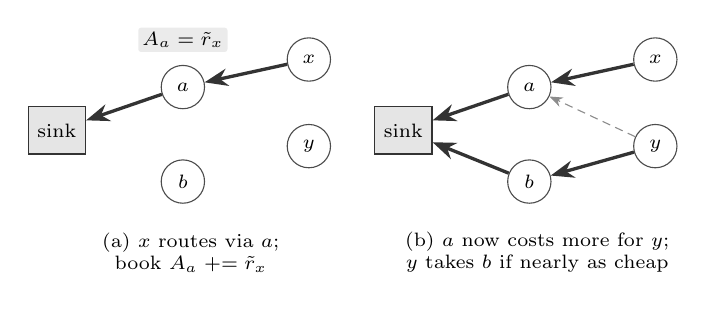
\begin{tikzpicture}[>=Stealth, node distance=1.2cm,
  nd/.style={circle, draw=black!70, fill=white, inner sep=1.4pt, minimum size=5.5mm, font=\scriptsize},
  sk/.style={rectangle, draw=black!80, fill=black!10, minimum size=6mm, font=\scriptsize}]
\begin{scope}
  \node[sk] (s) at (0,0) {sink};
  \node[nd] (a) at (1.6,0.55) {$a$};
  \node[nd] (b) at (1.6,-0.65) {$b$};
  \node[nd] (x) at (3.2,0.9) {$x$};
  \node[nd] (y) at (3.2,-0.2) {$y$};
  \draw[->, very thick, black!80] (x) -- (a);
  \draw[->, very thick, black!80] (a) -- (s);
  \node[font=\scriptsize, align=center] at (1.7,-1.55) {(a) $x$ routes via $a$;\\ book $A_a \mathrel{+}= \tilde r_x$};
  \node[font=\scriptsize, fill=black!8, rounded corners=1pt, inner sep=1.5pt] at (1.6,1.15) {$A_a=\tilde r_x$};
\end{scope}
\begin{scope}[xshift=4.4cm]
  \node[sk] (s2) at (0,0) {sink};
  \node[nd] (a2) at (1.6,0.55) {$a$};
  \node[nd] (b2) at (1.6,-0.65) {$b$};
  \node[nd] (x2) at (3.2,0.9) {$x$};
  \node[nd] (y2) at (3.2,-0.2) {$y$};
  \draw[->, very thick, black!80] (x2) -- (a2);
  \draw[->, very thick, black!80] (a2) -- (s2);
  \draw[->, densely dashed, black!45] (y2) -- (a2);
  \draw[->, very thick, black!80] (y2) -- (b2);
  \draw[->, very thick, black!80] (b2) -- (s2);
  \node[font=\scriptsize, align=center] at (1.7,-1.55) {(b) $a$ now costs more for $y$;\\ $y$ takes $b$ if nearly as cheap};
\end{scope}
\end{tikzpicture}
\caption{Within-round booking. Node $x$ is routed first and its traffic is booked on relay $a$. When $y$ is routed, $a$'s cost in Eq.~\eqref{eq:lest} has risen by the factor $1+\kappa A_a/\bar r$, so $y$ takes relay $b$ when its path is nearly as cheap. Battery-weighted Dijkstra would send both through $a$.}\label{fig:booking}
\end{figure}

\paragraph{Complexity} Each Dijkstra run on the dense graph costs $O(n^2)$, and at most one run is made per node that lacks a route when it is reached, so a round costs $O(n^3)$ in the worst case. In practice many nodes are fixed by earlier paths. The measured time is about 25~ms per round at $n=100$ on one CPU core, against under 1~ms for battery-weighted Dijkstra and about 0.2~s for one LP solve. Faster shortest-path algorithms~\cite{duan2025sorting} would change only this time, not the tree.

\subsection{Upper reference: the LP planner}\label{sec:lp-planner}
To measure what full flow optimisation adds, the sink re-solves the LP~\eqref{eq:lp-flow}--\eqref{eq:lp-energy} every round. The current batteries $E_i$ replace $E_0$, and each node generates $L\hat r_i$ bits per round, where $\hat r_i$ is its expected rate over the next 24 rounds. A small total-energy term breaks ties among equally long-lived plans:
\begin{equation}
\max\; T - \mu\textstyle\sum_{ij} f_{ij}\,\bigl(e_{\mathrm{tx}}(i,j)+e_{\mathrm{rx}}\bigr)/E_0, \qquad \mu=10^{-3}.\label{eq:tiebreak}
\end{equation}
The solution gives the fraction of each node's traffic to send to each next hop. In each round every node sends to one next hop, rotating among its LP next hops in proportion to those fractions (weighted round-robin), so each round is still a single tree. We call this configuration v2. Version v1 re-solves every 4 rounds without the tie-break. The rate $\hat r_i$ comes from additive Holt-Winters~\cite{holt2004forecasting,winters1960forecasting} with season length 24 ($\alpha=0.05$, $\beta=0$, $\gamma=0.1$; on Intel data $\gamma=0.3$), updated with the traffic the sink has just received. The ablation replaces it with a fixed historical mean. The LP is solved with HiGHS~\cite{huangfu2018highs}.

\subsection{Other reference methods}\label{sec:baselines}
\paragraph{MADII rebuild} No code was released, so the network, the reward, the metrics and the two-stage training of~\cite{yang2025madii} were rebuilt in PyTorch: an Informer encoder ($d_{\mathrm{model}}=128$, 2 layers, 4 heads), 1{,}000 episodes (300 imitation episodes from FCM, HBA and POA in rotation, then 700 $\varepsilon$-greedy), Adam with learning rate $10^{-4}$, and Double DQN~\cite{vanhasselt2016double} over 101 candidate next hops. The paper does not say how per-sensor Q-values form one training target. Averaging them before the loss let the network collapse to direct transmission, so each sensor's chosen value is regressed on the shared round return instead. Because all 100 sensors explore at once, the paper's $\varepsilon$ schedule ($1.0\to0.1$) randomises the whole network, so its shape is kept and scaled to $0.1\to0.01$. To check that these two choices do not explain the result, we also ran the paper's schedule and the paper's full model size (27.3~M parameters). Both landed in the same 8--11\% band (Section~\ref{sec:static}). MADII was trained on constant traffic and is not retrained for the time-varying scenarios.
\paragraph{EBR-DA, as specified} The node weight is $0.6(1-E/E_0)^2+0.4\,b^2$, with $b$ the buffer occupancy, over a hop tree with an 80~m radius~\cite{mahdi2018ebrda}, and each node forwards to its lightest neighbour one hop nearer the sink. Our model has no buffers, so occupancy is a node's traffic relative to the busiest node's. A node with no neighbour in range forwards to its nearest node nearer the sink (bridging); without bridging, isolated nodes die within a few rounds.
\paragraph{Dijkstra variants (negative results)} We also test the following variants:
\begin{itemize}[leftmargin=*]
  \item \emph{Predictive Dijkstra.} Each battery is reduced by a reserve for the extra load that Holt-Winters expects, $E_{\mathrm{eff},i}=\max(E_i-\lambda R_i,\,0.05E_i)$.
  \item \emph{Lifetime Dijkstra.} The cost is weighted by forecast load or by forecast rounds left.
  \item \emph{Receiver-weighted Dijkstra.} The receive cost is weighted by the receiver's battery.
  \item \emph{Price-guided Dijkstra.} The cost is scaled by the LP's dual energy prices, refreshed daily.
  \item \emph{RL warm-started from Dijkstra.} A 145-parameter network multiplies Eq.~\eqref{eq:battery} by $\exp(m_\theta(\phi_i))$ and is trained by PGPE~\cite{sehnke2010pgpe}. Its zero initial output makes the untrained policy exactly battery Dijkstra.
\end{itemize}
Each variant's settings were tuned on validation deployments (Section~\ref{sec:setup}).

\subsection{Characteristics of the evaluated algorithms}
Table~\ref{tab:characteristics} summarises what each evaluated router needs.

\begin{widetab}
\centering
\caption{Characteristics of the evaluated algorithms ($n=100$; times on one CPU core).}\label{tab:characteristics}
\footnotesize
\scriptsize\setlength{\tabcolsep}{3pt}\begin{tabularx}{\textwidth}{@{}L{0.17\textwidth}L{0.1\textwidth}XL{0.15\textwidth}L{0.1\textwidth}L{0.14\textwidth}L{0.09\textwidth}@{}}
\toprule
Algorithm & Decided by & Information used & Work per round & Training & Extra control bits & Time per round\\
\midrule
Min-energy Dijkstra & sink & positions & one Dijkstra & none & 0 & $<1$~ms\\
Battery-weighted Dijkstra & sink & + exact batteries & one Dijkstra & none & 0 & $<1$~ms\\
\textbf{LEST load-table Dijkstra} & sink & + 4-tier load per node & $\le n$ Dijkstra runs & none & 8/data packet + $2n$/round & $\approx25$~ms\\
LP planner v2 (reference) & sink & batteries + forecast rates & one LP (HiGHS) & HW fit & 0 & $\approx0.2$~s\\
Predictive / price-guided Dijkstra & sink & + forecast or LP prices & one Dijkstra (+ daily LP) & HW fit & 0 & $<1$~ms\\
EBR-DA~\cite{mahdi2018ebrda} & sink, per node rule & energy, buffer of neighbours & hop tree + local choice & none & 0 (not charged) & $<1$~ms\\
MADII~\cite{yang2025madii} & sink (centralised execution) & node states & Informer over $100\times101$ hops & 1{,}000 episodes & 0 & GPU in~\cite{yang2025madii}\\
\bottomrule
\end{tabularx}
\end{widetab}

\section{Evaluation protocol}\label{sec:setup}

\paragraph{Deployments and data splits} The held-out test set has 30 deployments (seeds 0--29) per scenario. All tuning uses separate validation deployments (seeds 500--511; for the RL warm start, 500--519), and RL training uses seeds of 1{,}000 and above. On the Intel Lab bench, batteries, Holt-Winters and the send-on-delta thresholds were set on the first 14 days. The test then ran once on 27 deployments starting every 8 hours in the later days. Every method sees the same deployments and traffic (A14).

\paragraph{Tuning} Each method's free settings were chosen on validation deployments, and only the best setting was run on the test set. For LEST Dijkstra, $\kappa\in\{0.03,\dots,10\}$ and two build orders were tried; nearest-first with $\kappa=1$ was best. The LEST tiers, band and trigger were taken unchanged from the original LEST design, not tuned. For the LP planner, re-solving every 8, 4, 2 and 1 rounds gave 86.9\%, 91.5\%, 94.1\% and 96.8\% of the oracle on validation, and the tie-break added up to 0.7 points. Two candidate changes were rejected on validation:
\begin{itemize}[leftmargin=*]
  \item Carrying round-robin credits across re-solves scored 81.1\%, because each re-solve already corrects past deviations.
  \item A burst-triggered re-solve fired on Poisson noise in 70--75\% of rounds.
\end{itemize}
The Dijkstra variants and EBR-DA's reconstructed cost were tuned the same way (32 settings for EBR-DA).

\paragraph{Metrics} The primary metric is FND as a percentage of the deployment's ceiling. We report its mean, its worst case over deployments, and wins/ties/losses (W/T/L) against battery-weighted Dijkstra, deployment by deployment. For the time-varying scenarios, the mean $S$ weights R, N and B equally. D is reported beside it.

\paragraph{Statistical testing} All comparisons are paired by deployment, so we use the two-sided Wilcoxon signed-rank test~\cite{wilcoxon1945}, as recommended for comparing algorithms over multiple problem instances~\cite{demsar2006}. The test makes no normality assumption, and lifetime ratios are bounded and skewed. Zero differences, where a method produces exactly the same lifetime, are counted as ties and dropped, following Wilcoxon. Within each family of comparisons the $p$-values are adjusted with the Holm procedure~\cite{holm1979}. As an effect size we report the matched-pairs rank-biserial correlation $r$~\cite{kerby2014}, which equals $+1$ when a method is better on every deployment. We use a significance level of 0.05 after adjustment.

\section{Results}\label{sec:results}

\subsection{Static traffic in MADII's setting}\label{sec:static}
\paragraph{Reproduction check} Table~\ref{tab:repro} compares our rebuild with MADII's printed results. The headline model matches, with 19.5 rounds to FND against the paper's 19. Two of the paper's baselines that we could implement exactly, HBA and POA, land within about 15\%. One mismatch remains: our FCM matches only at later death fractions. We also ran MADII exactly as published. With the paper's $\varepsilon$ schedule ($1.0\to0.1$), training episodes collapsed to 1--1.6 rounds once exploration began, and the held-out FND was 14.9 rounds (8.2\% of the ceiling). The paper's full model size (27.3~M parameters, evaluated at episode 200 of 1{,}000) reached 15.4 rounds (8.4\%). A model 90 times larger thus lands in the same band, and the rebuild matches the paper's own figure, so MADII's shortfall is not an artefact of our implementation choices.

\begin{table}[t]
\centering
\caption{Reproduction check against MADII's printed results (30 deployments; FND in rounds).}\label{tab:repro}
\footnotesize
\begin{tabular}{@{}L{0.5\linewidth}rrr@{}}
\toprule
Method & Rebuild & Printed~\cite{yang2025madii} & Ratio\\
\midrule
MADII (Informer) & 19.5 & 19 & 1.03\\
HBA clustering & 12.4 & 14 & 0.89\\
POA clustering & 10.9 & 13 & 0.84\\
FCM clustering & 5.4 & 19 & 0.28\\
\bottomrule
\end{tabular}
\end{table}

\paragraph{Every method against the optimum} Table~\ref{tab:static} and Fig.~\ref{fig:static} give the lifetime of each method as a percentage of the LP ceiling (mean $T^*=169.7$ rounds). Battery-weighted Dijkstra keeps every node alive for 151 rounds on average, 88.4\% of the optimum, against 19.5 rounds (11.1\%) for MADII: about $8\times$ longer, with no training. It differs from min-energy Dijkstra (24.3\%) by a single factor, the battery weighting. Every one of the 30 deployments under battery Dijkstra lies between 80.8\% and 92.6\% of the optimum, whereas MADII stays between 3.9\% and 19.3\%. The gap therefore holds deployment by deployment, not only on average. LP-flow re-solved every 4 rounds reaches 94.5\%. RL warm-started from battery Dijkstra gains 0.5 points, which is not significant ($p=0.24$).

\begin{widetab}
\centering
\caption{Static traffic in MADII's setting: lifetime against the provable optimum (30 held-out deployments). W/T/L and $p$ against battery-weighted Dijkstra (Wilcoxon signed-rank).}\label{tab:static}
\footnotesize
\setlength{\tabcolsep}{4pt}
\begin{tabular}{@{}L{0.40\textwidth}rrrl@{}}
\toprule
Method & FND & \% of $T^*$ & Worst \% & W/T/L, $p$\\
\midrule
\inputtab{body/tab_static.tex}
\bottomrule
\end{tabular}
\end{widetab}

\begin{figure}[t]
\centering
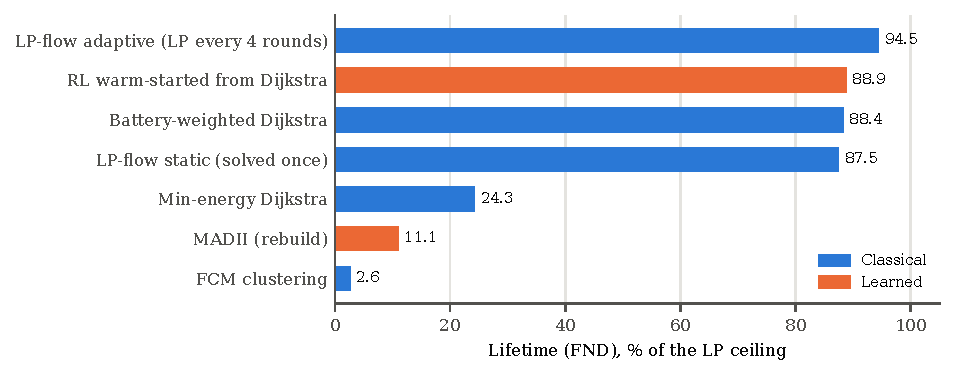
\includegraphics[width=\linewidth]{figs/static.pdf}
\caption{Static traffic in MADII's setting: mean lifetime to first node death as a percentage of the LP ceiling (30 held-out deployments).}\label{fig:static}
\end{figure}

\subsection{Time-varying traffic}\label{sec:dynamic}
Table~\ref{tab:dynamic} and Fig.~\ref{fig:ladder} report the time-varying scenarios. LEST load-table Dijkstra reaches 90.5\% of the oracle, against 85.0\% for battery-weighted Dijkstra. It wins 118 of the 120 deployments across R, N, B and D, and it gains in every scenario, including the pattern shift that nothing was tuned on (90.0\% against 83.0\%). It closes about half of the gap between battery Dijkstra and the LP planner with no solver and no training. Sharing load through the 4-tier LEST table, with its overhead charged, costs 0.3 points against exact loads (90.5\% against 90.8\%). The LP planner v2 reaches 97.0\% and beats battery Dijkstra on all 120 deployments, with a worst case of 92.1\% against 74.3\%. MADII, trained on constant traffic, stays at 13--16\%, and EBR-DA as specified at 14\%. The best of five ways of adding prediction or tuning to Dijkstra, LP-price guidance, gains 1.0 point, and the others stay at or below battery Dijkstra.

\begin{widetab}
\centering
\caption{Time-varying traffic: lifetime as a percentage of the oracle (30 held-out deployments per scenario; R: daily surge, N: constant, B: bursts, D: pattern shift). Mean $S$ weights R, N and B equally; Worst is over those 90 deployments; D is not tuned on. W/T/L against battery-weighted Dijkstra over all 120 deployments.}\label{tab:dynamic}
\footnotesize
\setlength{\tabcolsep}{4pt}\begin{tabular}{@{}L{0.33\textwidth}rrrrrrr@{}}
\toprule
Method & R & N & B & Mean $S$ & Worst & D & W/T/L\\
\midrule
\inputtab{body/tab_dynamic.tex}
\bottomrule
\end{tabular}
\end{widetab}

\begin{figure}[t]
\centering
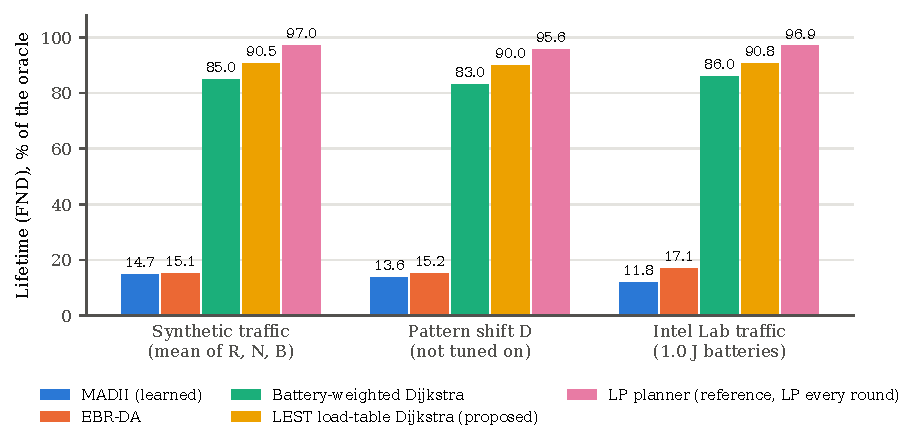
\includegraphics[width=\linewidth]{figs/ladder.pdf}
\caption{Lifetime as a percentage of the oracle on synthetic traffic, under a pattern shift and on real Intel Lab traffic.}\label{fig:ladder}
\end{figure}

\subsection{Ablation of LEST load-table Dijkstra}\label{sec:ablation}
Table~\ref{tab:ablation} removes each part of the method in turn.
\begin{itemize}[leftmargin=*]
  \item \textbf{Load only.} Without the battery weight, the load table alone reaches 45.1\%. It spreads traffic evenly but keeps relaying through nodes that are running out.
  \item \textbf{Energy only.} Without the load table the method is battery-weighted Dijkstra, at 85.0\%. It protects weak nodes but lets many nodes pile onto the same relay.
  \item \textbf{Energy in tiers.} Compressing energy into LEST tiers as well lowers validation lifetime to 43.8\% with the original trigger. A slowly draining battery never moves by more than the 0.05 band between two reports, so its tier never changes (zero tier changes in a test run). With a standard Schmitt trigger it reaches 79.2\%, and it needs 32 levels or more to recover 89\%.
  \item \textbf{Load in tiers.} The original trigger works for load: rates jump from round to round, so a tier changes in only 0.19\% of node-rounds. Finer load tables (8 or 16 levels) gain at most 0.2 points.
\end{itemize}
EBR-DA also mixes energy and load~\cite{mahdi2018ebrda}, but with a squared term that is linear in energy and over a minimum-hop tree. It reaches 15\% as specified. With its cost retuned on our bench it reaches 50.3\%, still far below the sharp $E_0/E_i$ weight combined with load booked within the round.

\begin{table}[t]
\centering
\caption{Ablation of LEST load-table Dijkstra (\% of the oracle; held-out: mean of R, N, B over 90 deployments; validation: seeds 500--511). Control bits per alive node per round in the last column.}\label{tab:ablation}
\footnotesize
\setlength{\tabcolsep}{4pt}
\begin{tabular}{@{}L{0.5\linewidth}rrr@{}}
\toprule
Variant & Held-out & Validation & Ctrl bits\\
\midrule
\textbf{Exact energy + LEST load (proposed)} & \textbf{90.5} & 90.7 & 300\\
Exact energy + exact load & 90.8 & 91.1 & 100\\
Exact energy only (battery Dijkstra) & 85.0 & 84.6 & 100\\
Load only (no battery weight) & 45.1 & 46.7 & 100\\
Exact energy + LEST load, Schmitt trigger & -- & 90.4 & 300\\
Exact energy + 8 / 16-level load & -- & 90.9 / 90.7 & 400 / 500\\
Energy also in 4 tiers, original trigger & -- & 43.8 & 400\\
Energy also in 4 tiers, Schmitt trigger & -- & 79.2 & 400\\
Energy also in 32 / 256 levels & -- & 89.0 / 89.1 & 1{,}200 / 1{,}600\\
EBR-DA as specified~\cite{mahdi2018ebrda} & 13.9 & -- & 100\\
EBR-DA cost, retuned on this bench & 50.3 & 53.3 & 100\\
\bottomrule
\end{tabular}
\end{table}

\subsection{What prediction adds}\label{sec:prediction}
\paragraph{To the LP planner} With the same v2 planner, a fixed historical rate reaches 96.5\% against 97.0\% with Holt-Winters. The difference is $+0.7$ points under surges (17/6/7, $p=0.047$ unadjusted, $p=0.19$ after Holm correction), zero with constant traffic, and not significant under bursts or the pattern shift. The forecast's clearest benefit is the worst case (92.1\% against 84.8\%). Holt-Winters already matches a perfect forecast (96.9\%), so a better forecaster could not add more. The gain comes from the planner: moving from v1 (every 4 rounds) to v2 (every round) adds 6.6, 1.1, 7.8 and 7.7 points in R, N, B and D. Re-solving from measured batteries corrects a wrong rate through the batteries themselves. What matters is a rate averaged over a full day. A reactive LP that plans with the last 4 rounds' traffic collapses to 50--53\% under surges, and persistence to 13\%.

\paragraph{To Dijkstra} Prediction, lifetime weighting, exponent tuning and LP prices all stay within about $\pm1$ point of battery Dijkstra (Table~\ref{tab:dynamic}). Stronger battery exponents are worse: $\alpha=2$, 5, 20 and 50 give 77.4\% down to 10.7\% on validation. LP prices fed back every round collapsed to 6--18\% on validation. A tracing study explains predictive Dijkstra's loss under surges. One hour before each surge, the 20\% of nodes with the highest forecast are exactly the hotspot nodes in every deployment, so the forecast senses the pattern correctly. Predictive Dijkstra does move relay traffic off those nodes before the surge (from 30.2\% to 28.2\% of relayed packets). Once the surge starts, however, the reserve vanishes, the spared nodes look rich, their relay share rises (43.6\% to 46.8\%), and a hotspot node dies first in 67\% of deployments against 47\%. Battery Dijkstra already charges every relay its energy per packet divided by its battery. Any further per-node signal moves whole subtrees onto neighbours, which then die first. LEST Dijkstra avoids this because its booking is incremental within the round.

\subsection{Real traffic: Intel Berkeley Lab}\label{sec:intel}
Table~\ref{tab:intel} shows that the ranking found on synthetic traffic holds on real traffic. At $E_0=1.0$~J, LEST Dijkstra reaches 90.8\% against 86.0\% for battery Dijkstra (16/7/4), and the LP planner reaches 96.9\%. EBR-DA reaches 17.1\% and MADII 11.8\%. The forecast is far more accurate than the historical mean here (next-day rate error 0.52 against 1.03 packets per mote-hour), yet the lifetime difference is only 0.3 points, and its visible benefit is again the worst case (88.8\% against 79.9\%). At $E_0=1.5$~J, about half the deployments outlive the dataset and count as ties, so the 1.0~J run is the cleaner comparison.

\begin{widetab}
\centering
\caption{Intel Lab traffic: lifetime as a percentage of the oracle (27 test deployments). W/T/L against battery-weighted Dijkstra.}\label{tab:intel}
\footnotesize
\setlength{\tabcolsep}{4pt}\begin{tabular}{@{}L{0.36\textwidth}rrrrrr@{}}
\toprule
& \multicolumn{3}{c}{$E_0=1.0$~J} & \multicolumn{3}{c}{$E_0=1.5$~J}\\
\cmidrule(lr){2-4}\cmidrule(l){5-7}
Method & Mean & Worst & W/T/L & Mean & Worst & W/T/L\\
\midrule
\inputtab{body/tab_intel.tex}
\bottomrule
\end{tabular}
\end{widetab}

\subsection{Statistical tests}\label{sec:stats}
Table~\ref{tab:wilcoxon} reports the paired Wilcoxon signed-rank tests for the main comparisons, and Fig.~\ref{fig:paired} shows the deployment-by-deployment pairs behind the central one.
\begin{itemize}[leftmargin=*]
  \item \textbf{LEST Dijkstra against battery Dijkstra.} LEST Dijkstra is better on time-varying traffic (median $+4.6$ points, $p_{\mathrm{Holm}}=2.2\times10^{-20}$, $r=+1.00$) and on Intel Lab traffic (median $+0.5$, $p_{\mathrm{Holm}}=0.005$, $r=+0.81$).
  \item \textbf{LP planner against LEST Dijkstra.} The LP planner is better again in both settings.
  \item \textbf{LEST against exact loads.} The 4-tier table loses a small but significant 0.5 points against exact loads on synthetic traffic ($p=6.4\times10^{-4}$), the price of sharing load in 2 bits.
  \item \textbf{Prediction and learning on Dijkstra.} Predictive Dijkstra is significantly \emph{worse} than battery Dijkstra on synthetic traffic ($p=0.007$). RL warm-started from Dijkstra is not significantly different from it ($p=0.24$).
\end{itemize}
Every adjusted $p$ for MADII and EBR-DA is below $10^{-6}$, with $r=-1$.

\begin{widetab}
\centering
\caption{Paired Wilcoxon signed-rank tests (two-sided). Mean and median are the paired differences, first method minus second, in points of the oracle percentage. Holm adjustment is applied within each setting's family of comparisons; $r$ is the matched-pairs rank-biserial correlation.}\label{tab:wilcoxon}
\footnotesize
\setlength{\tabcolsep}{4pt}\begin{tabular}{@{}L{0.30\textwidth}rrrrrr@{}}
\toprule
Comparison & Mean & Median & W/T/L & $p$ & $p_{\mathrm{Holm}}$ & $r$\\
\midrule
\inputtab{body/tab_wilcoxon.tex}
\bottomrule
\end{tabular}
\end{widetab}

\begin{figure}[t]
\centering
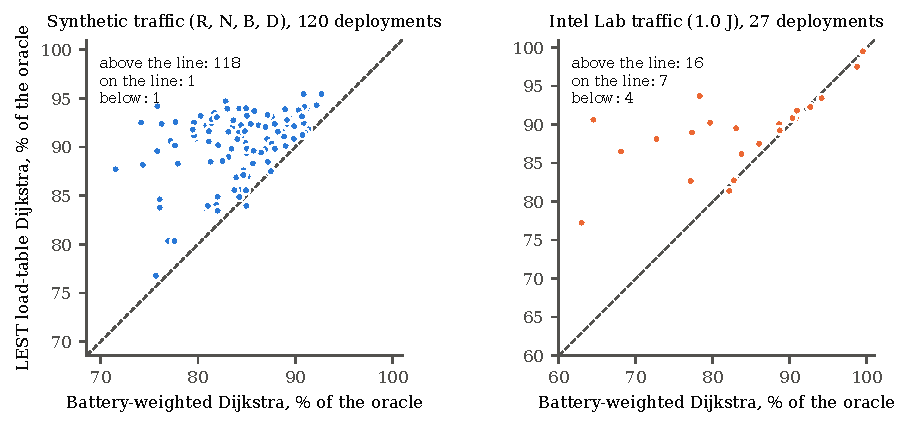
\includegraphics[width=\linewidth]{figs/paired.pdf}
\caption{Deployment-by-deployment lifetime of LEST load-table Dijkstra against battery-weighted Dijkstra. Points above the dashed line are deployments where LEST Dijkstra lives longer.}\label{fig:paired}
\end{figure}

\subsection{Traffic metrics and computation}\label{sec:computation}
Lifetime is not bought at the expense of delivery (Table~\ref{tab:traffic}). In MADII's static setting, the delivery ratio is about 99\% for every router. LEST Dijkstra delivers more data by the time half the nodes are dead (HND) than battery Dijkstra, and more per joule. MADII delivers 2.7 times less data by HND and about half as much per joule. Its one advantage is shorter paths (2.61 hops), obtained from long direct links that drain batteries. Our rebuild delivers 25{,}349~kbit by HND against the paper's printed 25{,}708, a further check on the reproduction. In computation, battery Dijkstra needs under 1~ms per round, LEST Dijkstra about 25~ms and the LP planner about 0.2~s, all at the mains-powered sink, while MADII needs 1{,}000 training episodes before use (Table~\ref{tab:characteristics}).

\begin{table}[t]
\centering
\caption{Traffic metrics in MADII's setting (constant traffic, 30 deployments). HND: rounds until half the nodes are dead. This run uses the time-varying simulator with constant traffic. The classical routers give the same FND as in Table~\ref{tab:static}, but the MADII rebuild gives 27.3 rounds rather than 19.5. Either value is below 17\% of the ceiling.}\label{tab:traffic}
\footnotesize
\setlength{\tabcolsep}{3pt}
\begin{tabular}{@{}L{0.3\linewidth}rrrrrr@{}}
\toprule
Router & FND & HND & kbit by HND & kbit/J & Deliv. & Hops\\
\midrule
LP planner v2 & 167.7 & 170.7 & 67{,}475 & 1{,}355 & 99.1\% & 3.23\\
\textbf{LEST Dijkstra} & 157.8 & 163.7 & 64{,}686 & 1{,}306 & 99.1\% & 3.34\\
Battery Dijkstra & 151.4 & 162.9 & 63{,}843 & 1{,}286 & 98.9\% & 3.53\\
Min-energy Dijkstra & 42.5 & 159.1 & 55{,}735 & 1{,}336 & 99.3\% & 3.96\\
MADII rebuild & 27.3 & 73.3 & 25{,}349 & 681 & 99.2\% & 2.61\\
MADII, printed~\cite{yang2025madii} & 19 & 89 & 25{,}708 & -- & -- & --\\
\bottomrule
\end{tabular}
\end{table}

\section{Discussion}\label{sec:discussion}

\paragraph{Why MADII falls short} There are three reasons, and none of them requires a bug in our rebuild.
\begin{itemize}[leftmargin=*]
  \item \textbf{The imitation stage does not teach the expert's behaviour.} It only fills the replay memory with expert decisions for Q-learning, and the network is never trained to reproduce them. Consistent with this, a run that used battery Dijkstra (a 151-round expert) as the imitation source fell from 7.6 to 4.4 rounds between episodes 25 and 50; this run was stopped early.
  \item \textbf{The Informer has nothing to forecast.} It was designed for long time-series forecasting~\cite{zhou2021informer}. MADII feeds it a single snapshot of 101 nodes and asks it to route, and its sparse attention gains nothing at that size.
  \item \textbf{No baseline revealed the gap.} MADII is compared only with clustering, metaheuristic and learned methods, so the distance to shortest-path routing and to the optimum went unnoticed.
\end{itemize}
The broader lesson concerns evaluation practice. A learned router should be reported against a battery-weighted shortest-path router and against a provable ceiling. Both are cheap to compute, and together they place any new method on an absolute scale.

\paragraph{Why coordination, and why exact energy} Battery-weighted Dijkstra already captures most of the lifetime available from a single tree per round. What it lacks is coordination: nodes choose independently and overload shared relays. Booking load within the round supplies that coordination without a solver. Each extra unit of booked traffic raises a relay's cost smoothly, so close decisions tip towards alternatives while necessary relays are still used. The ablation shows that the two signals correct each other. Energy without load lets nodes pile onto one relay, and load without energy keeps relaying through nearly empty nodes. Energy must stay exact for a different reason: it drains slowly, so any reporting rule that is robust to noise, such as LEST's hysteresis trigger, freezes it. Load jumps from round to round and survives compression into 2 bits. The same freeze explains an observation from our earlier fuzzy-Q project, where every node remained in the same energy tier for the whole run.

\paragraph{When to use which router} If a sink can afford one LP solve per round (about 0.2~s at $n=100$), the LP planner is the best choice, at 97\% of the oracle. If it cannot, LEST Dijkstra reaches about 90\% with shortest paths alone, and battery Dijkstra about 85\% with a single Dijkstra run. A traffic forecast is a small robustness refinement for the planner and does not help Dijkstra. In this setting, learning brings no benefit we could measure.

\subsection{Threats to validity}\label{sec:threats}
\paragraph{Internal validity} MADII is our rebuild from the paper's text. It reproduces the headline lifetime and delivered data, but it is not the authors' code, which has not been released; we have requested it. Two harnesses give MADII different FND values (19.5 and 27.3 rounds); both are below 17\% of the ceiling, and the classical routers agree across harnesses. EBR-DA is evaluated outside the aggregation setting it was designed for, with buffer occupancy approximated by load. All tuned settings were chosen on validation deployments, and the test sets were run once.
\paragraph{Construct validity} FND is one of several lifetime definitions. We also report 10\%, 25\% and 50\% dead, delivered data and energy efficiency (Table~\ref{tab:traffic}), and the ranking is the same.
\paragraph{External validity} The radio model is the idealised one used by MADII (A3--A6): no collisions, no lossy links, no barriers and no idle-listening energy. Absolute percentages may shift under a packet-level MAC with retransmissions. Lossy links would raise the cost of long hops and of busy relays alike, which we expect to favour load-aware routing, but this has not been tested. The synthetic traffic models are designed by us. The Intel layout is scaled, its traffic is derived from readings rather than measured, and test deployments overlap in time. Networks of 54 and 100 nodes are tested; the LP grows with the square of $n$, and LEST Dijkstra's worst case with its cube. Both LEST Dijkstra and the LP planner compute routes at the sink. A fully distributed variant, in which every node computes the same tree from a shared snapshot, would also need every battery level at every node, and it has not been tested.

\section{Conclusion}\label{sec:conclusion}

Measured against a provable optimum, energy-efficient WSN routing falls into clear levels. A recent multi-agent DRL router and a published energy-and-load router reach about 15\% of the ceiling. Battery-weighted Dijkstra reaches about 85\% with no training. LEST load-table Dijkstra reaches about 90\% with no solver. An LP planner re-solved every round reaches 97\%. LEST load-table Dijkstra builds each round's tree node by node, books every source's traffic on its path, and shares load through a 4-tier table whose overhead it pays for. It wins 118 of 120 time-varying deployments against battery Dijkstra, and the ranking holds on real Intel Lab traffic. Prediction adds half a point to the planner and nothing to Dijkstra, and learning adds no measurable gain. For lifetime routing in this setting, coordination and planning are what matter.

Future work will cover four directions:
\begin{itemize}[leftmargin=*]
  \item a distributed LEST Dijkstra, in which every node computes the same tree from a shared snapshot of energy and load;
  \item a packet-level evaluation with lossy links taken from the Intel connectivity data, collisions and retransmissions, together with networks of 200--500 nodes;
  \item further published learned baselines, including MADII retrained on time-varying traffic or the authors' code if it is released;
  \item traffic with stronger drift or weekly cycles, where prediction may matter more.
\end{itemize}


\section*{Data Availability}
The simulator, every router, the result files and the scripts that regenerate every table and figure are available at [repository URL]. The Intel Berkeley Lab data are publicly available~\cite{intellab2004}.

\bibliographystyle{IEEEtran}
\bibliography{refs}

\end{document}
